% ============================================================
% Chapitre 6 : Réalisation, Tests et Déploiement
% ============================================================

\section{Introduction}

À l'issue des phases d'analyse des besoins et de conception architecturale, ce chapitre décrit
la concrétisation technique de la plateforme \textbf{RevMine}. Il couvre l'ensemble du processus
de réalisation~: de la mise en place de la culture DevOps et de l'environnement de développement
jusqu'à l'implémentation des différents modules du système, en passant par la stratégie de test
et le déploiement continu.

L'objectif de cette phase est de produire une application capable de centraliser la configuration
des espaces de travail, de collecter les données issues des plateformes de gestion de code, de les
nettoyer et de les structurer, puis de générer des analyses visuelles exploitables. Pour répondre
à ces exigences, une architecture microservices a été adoptée, avec une séparation claire des
responsabilités entre le service de passerelle d'API, les services métier, les mécanismes de
communication asynchrone et les composants d'infrastructure.

Ce chapitre présente successivement la culture DevOps adoptée, la gestion de projet,
l'environnement de réalisation, les technologies retenues, l'implémentation des microservices
backend et de l'interface frontend, les mécanismes de communication inter-services, les mesures
de sécurité, ainsi que la stratégie de test et le pipeline de livraison continue.

% ============================================================
\section{Culture DevOps}
% ============================================================

\subsection{Principes généraux}

Le développement de RevMine s'inscrit dans une culture \textbf{DevOps}, paradigme qui rapproche
les équipes de développement (\textit{Dev}) et d'exploitation (\textit{Ops}) afin de livrer des
logiciels de manière plus rapide, plus fiable et plus itérative \parencite{bass2015devops}. DevOps
repose sur un ensemble de pratiques couvrant l'intégralité du cycle de vie du logiciel~: codage,
construction, test, déploiement et surveillance. Ce cycle est souvent représenté sous la forme
d'une boucle infinie (symbole $\infty$) illustrant la continuité et l'amélioration permanente du
processus, comme illustré à la Figure~\ref{fig:devops-cycle}.

\begin{figure}[H]
    \centering
    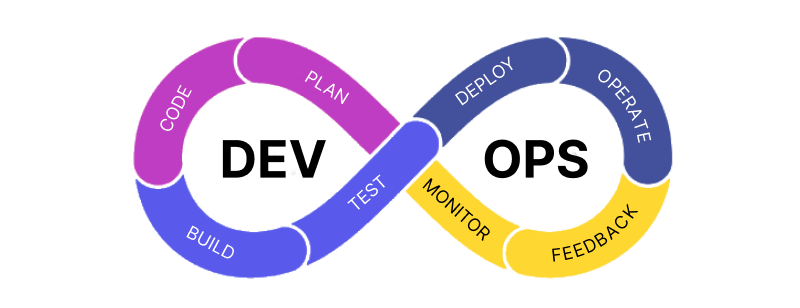
\includegraphics[width=0.75\textwidth]{assets/devops_cycle.png}
    \caption{Cycle de vie DevOps -- boucle d'amélioration continue}
    \label{fig:devops-cycle}
\end{figure}

Concrètement, les pratiques DevOps retenues pour RevMine se déclinent ainsi~:

\begin{itemize}
    \item \textbf{Code}~: développement collaboratif sur GitLab avec revue systématique de chaque
          contribution via des Merge Requests~;
    \item \textbf{Build}~: construction automatisée des images Docker à chaque fusion sur la
          branche principale~;
    \item \textbf{Test}~: exécution automatique des tests unitaires, d'intégration et de qualité
          statique à chaque commit via le pipeline GitLab CI~;
    \item \textbf{Déploiement}~: orchestration de l'ensemble des services applicatifs et
          d'infrastructure~;
    \item \textbf{Surveillance}~: collecte et visualisation des journaux applicatifs et des erreurs.
\end{itemize}

\subsection{Méthodologie Scrum}

La gestion du projet s'est inspirée de la méthode \textbf{Scrum}, cadre agile structurant le
développement en itérations courtes et régulières appelées \textit{sprints}
\parencite{schwaber2020scrum}. Les sprints ont été fixés à une durée d'une semaine, permettant
des cycles de livraison rapides et une adaptation continue aux retours obtenus.

Le projet RevMine a été réalisé en \textbf{binôme}, ce qui a nécessité une coordination étroite
tout au long du développement. Deux cadences de réunion ont structuré le suivi du projet~:

\begin{itemize}
    \item \textbf{Réunions hebdomadaires (chaque jeudi)}~: ces séances servaient à la fois de
          revue de sprint et de planification. Nous y présentions les fonctionnalités développées
          au cours de la semaine, levions les blocages techniques et définissions les objectifs du
          sprint suivant. La régularité de ces rendez-vous a permis une adaptation rapide aux
          retours et un alignement continu entre les réalisations et les attentes du projet~;
    \item \textbf{Réunions mensuelles}~: À un rythme mensuel, l'équipe présentait l'avancement global du projet devant l'équipe de recherche de l'\textbf{ETS} (École de Technologie Supérieure). Ces réunions constituaient une opportunité précieuse d'obtenir un retour critique de la part de professionnels du métier, apportant un regard extérieur sur les choix fonctionnels et techniques de la plateforme. Les observations formulées lors de ces séances ont contribué à affiner certaines orientations du projet et à valider la pertinence des fonctionnalités développées au regard des besoins réels du terrain.

\end{itemize}

Cette double cadence de suivi -- hebdomadaire pour le pilotage opérationnel et mensuelle pour la
validation avec avec l'équipe de recherche -- a favorisé une livraison incrémentale des fonctionnalités et une
détection précoce des écarts tout au long du développement.

\subsection{Politique de gestion des branches}

Afin de maintenir la lisibilité de l'historique Git et de sécuriser l'intégrité de la branche
principale, une \textbf{politique de branches} rigoureuse a été adoptée, s'inspirant du
\textit{Feature Branch Workflow} \parencite{atlassian2023gitflow}. Ce modèle préconise que chaque
nouvelle unité de travail -- fonctionnalité, correction ou amélioration -- soit développée dans
une branche dédiée, isolant ainsi les modifications en cours des livrables stables.

\subsubsection*{Justification du choix}

Plusieurs alternatives ont été envisagées. Le modèle \textit{Gitflow} classique, avec ses branches
\texttt{develop}, \texttt{release} et \texttt{hotfix}, s'avère surdimensionné pour un binôme
réalisant des livraisons continues sans gestion de versions numérotées. Le \textit{Trunk-Based
Development}, où tous les développeurs poussent directement sur la branche principale, présente un
risque élevé d'instabilité pour un projet en construction active. Le \textit{Feature Branch
Workflow} représente le meilleur compromis~: chaque fonctionnalité est isolée dans sa propre
branche, ce qui protège la branche principale tout en restant simple à opérer à deux.

\subsubsection*{Convention de nommage}

La convention de nommage suivante a été appliquée de manière systématique~:

\begin{itemize}
    \item \texttt{feature/<nom-fonctionnalité>}~-- développement d'une nouvelle fonctionnalité~;
    \item \texttt{fix/<description-du-bug>}~-- correction d'un défaut~;
    \item \texttt{refactor/<module>}~-- refactorisation d'un composant existant~;
    \item \texttt{test/<service>}~-- ajout ou mise à jour de tests~;
    \item \texttt{docs/<sujet>}~-- modification de la documentation.
\end{itemize}

Ce nommage structuré présente plusieurs avantages~: il permet d'identifier instantanément la
nature et la portée d'une branche, facilite le filtrage et la recherche dans l'historique Git,
et réduit les risques de confusion lors des revues de code. Toutes les branches sont créées
depuis \texttt{main} et fusionnées après revue via une Merge Request. Aucun commit direct sur
la branche principale n'est autorisé, garantissant ainsi la stabilité permanente du code de
référence.

% ============================================================
\section{Gestion de projet}
% ============================================================

\subsection{Tableau Kanban}

La gestion des tâches a été assurée à l'aide du tableau \textbf{Kanban} (littéralement
\og{}panneau visuel\fg{} en japonais) intégré à GitLab. Cet outil offre une représentation
visuelle de l'état d'avancement de chaque tâche, permettant aux deux membres du binôme
d'identifier rapidement les blocages et de prioriser les efforts. Chaque fonctionnalité,
correction ou amélioration a été formalisée sous forme d'\textit{issue}, puis suivie tout au
long de son cycle de vie grâce à cinq statuts distincts et un système d'étiquettes structuré.

\subsubsection*{Statuts du tableau}

Cinq statuts ont été définis pour refléter fidèlement l'avancement de chaque tâche~:

\begin{itemize}
    \item \textbf{À faire} (\textit{To Do})~: la tâche est identifiée et planifiée pour le sprint
          en cours, mais le développement n'a pas encore débuté~;
    \item \textbf{En cours} (\textit{In Progress})~: le développement est actif~; une seule
          personne du binôme est responsable de la tâche à ce stade afin d'éviter les conflits
          de travail~;
    \item \textbf{En revue} (\textit{Under Review})~: le développement est terminé et une Merge
          Request a été ouverte~; la tâche est en attente de revue par l'autre membre du binôme
          avant intégration~;
    \item \textbf{Bloquée} (\textit{Blocked})~: la tâche ne peut pas avancer en raison d'une
          dépendance non résolue ou d'un blocage technique~; ce statut permet de signaler
          rapidement les obstacles et de les traiter en priorité lors des points hebdomadaires~;
    \item \textbf{Clôturée} (\textit{Closed})~: la tâche est terminée, revue, intégrée dans la
          branche principale et validée.
\end{itemize}

\subsubsection*{Système d'étiquettes}

Chaque issue est enrichie d'un ensemble d'étiquettes permettant de la caractériser selon plusieurs
dimensions~:

\begin{itemize}
    \item \textbf{Composant}~: \texttt{frontend}, \texttt{backend} ou \texttt{ai}, indiquant la
          couche technique concernée~;
    \item \textbf{Nature}~: \texttt{feat} (nouvelle fonctionnalité) ou \texttt{bug} (correction
          d'un défaut)~;
    \item \textbf{Priorité}~: niveau d'urgence parmi \texttt{low}, \texttt{medium} et
          \texttt{high}, facilitant l'arbitrage lors de la planification du sprint~;
    \item \textbf{Sprint}~: étiquette indiquant le sprint auquel la tâche est rattachée, assurant
          la traçabilité de la charge de travail par itération.
\end{itemize}

La Figure~\ref{fig:kanban} illustre le tableau Kanban tel qu'utilisé dans GitLab, avec les
différentes colonnes de statut et le système d'étiquettes.

\begin{figure}[H]
    \centering
    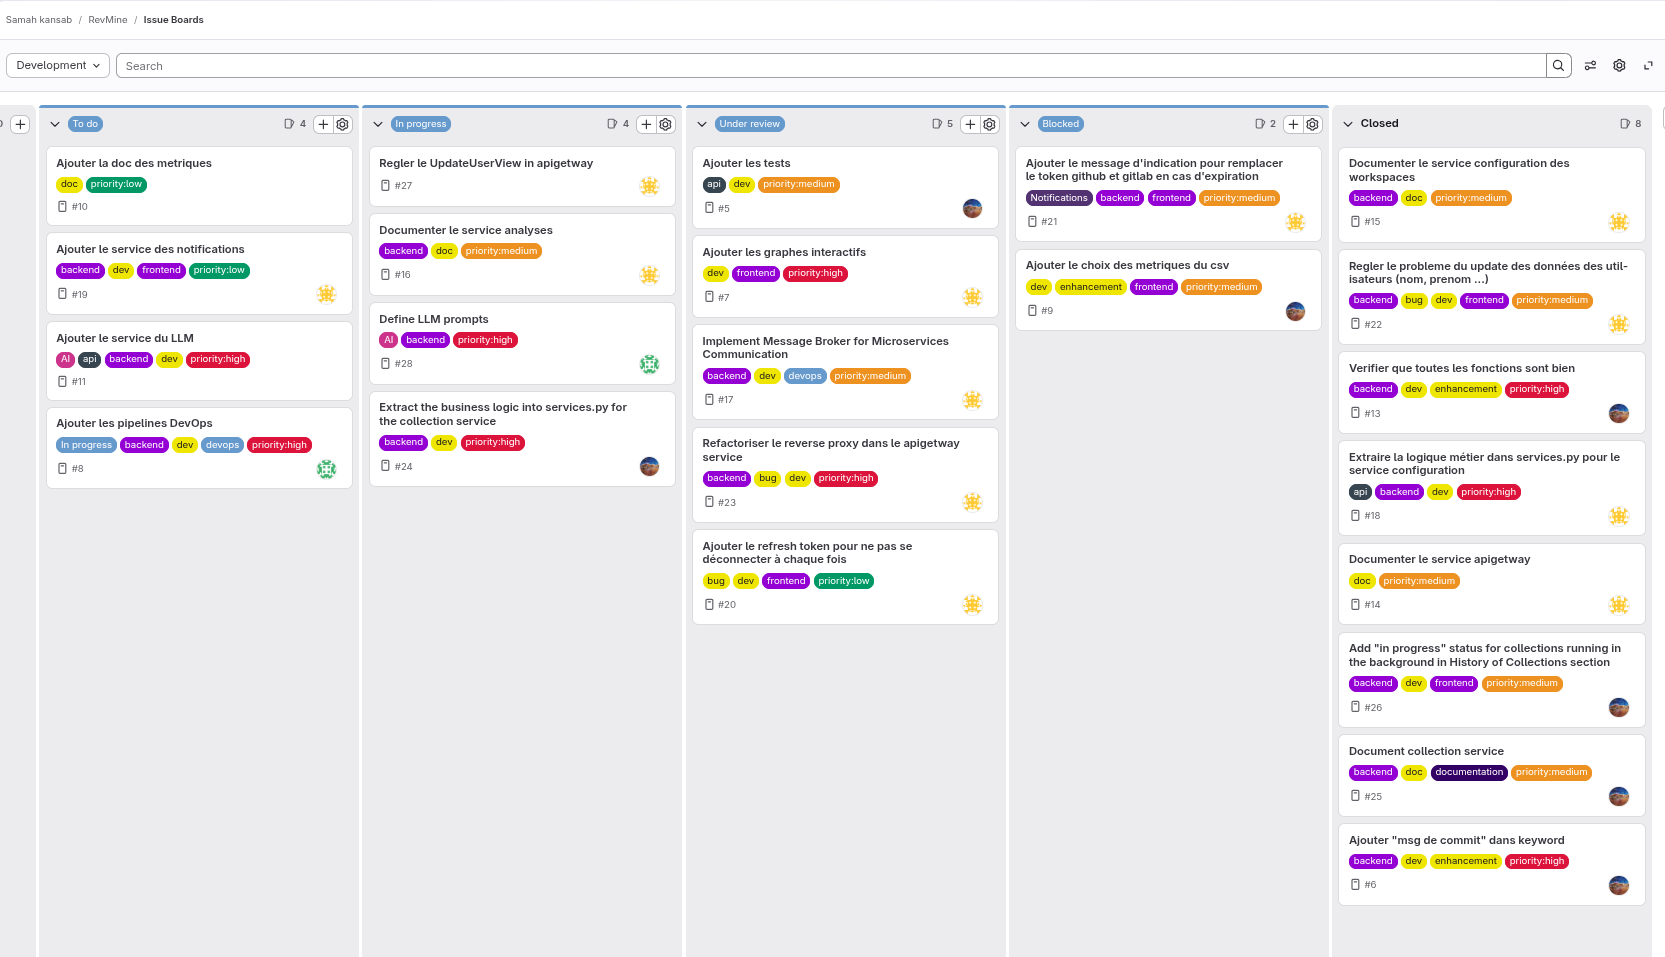
\includegraphics[width=0.95\textwidth]{captures/kanban_board.png}
    \caption{Tableau Kanban GitLab utilisé pour le suivi des tâches du projet RevMine}
    \label{fig:kanban}
\end{figure}

\subsection{Revue de code}
 
La branche \texttt{main} du dépôt GitLab a été configurée en mode \textbf{protégé}~: aucun
commit direct n'y est autorisé, et toute intégration passe obligatoirement par une
\textbf{Merge Request} (MR). Ce mécanisme constitue le point de contrôle central de la qualité
du code tout au long du développement.
 
Selon la nature et la portée de la tâche, deux niveaux de revue ont été appliqués~:
 
\begin{itemize}
    \item \textbf{Revue croisée}~: pour les fonctionnalités significatives, les modifications
          d'architecture ou les corrections de bugs critiques, la MR est soumise à l'examen de
          l'autre membre du binôme et, lorsque pertinent, à l'encadrant. La revue porte sur la
          correction fonctionnelle, la lisibilité du code, le respect des conventions de nommage
          et de structure, ainsi que l'absence de régressions. Les remarques sont formulées
          directement sous forme de commentaires inline dans GitLab, favorisant un échange
          précis et traçable~;
    \item \textbf{Auto-approbation}~: pour les tâches mineures -- corrections typographiques
          dans la documentation, ajustements de configuration, mises à jour de dépendances
          sans impact fonctionnel -- le membre ayant ouvert la MR procède lui-même à son
          approbation (\textit{self-approve}), afin de ne pas bloquer inutilement le flux de
          travail sur des changements à faible risque.
\end{itemize}
 
Cette politique à deux vitesses permet de concilier rigueur et agilité~: les modifications
sensibles bénéficient d'un regard extérieur systématique, tandis que les tâches routinières
ne génèrent pas de délais d'attente superflus. La Figure~\ref{fig:code-review} illustre un
exemple de revue de code réalisée sur une Merge Request, avec des commentaires formulés
directement sur les lignes concernées.
 
\begin{figure}[H]
    \centering
    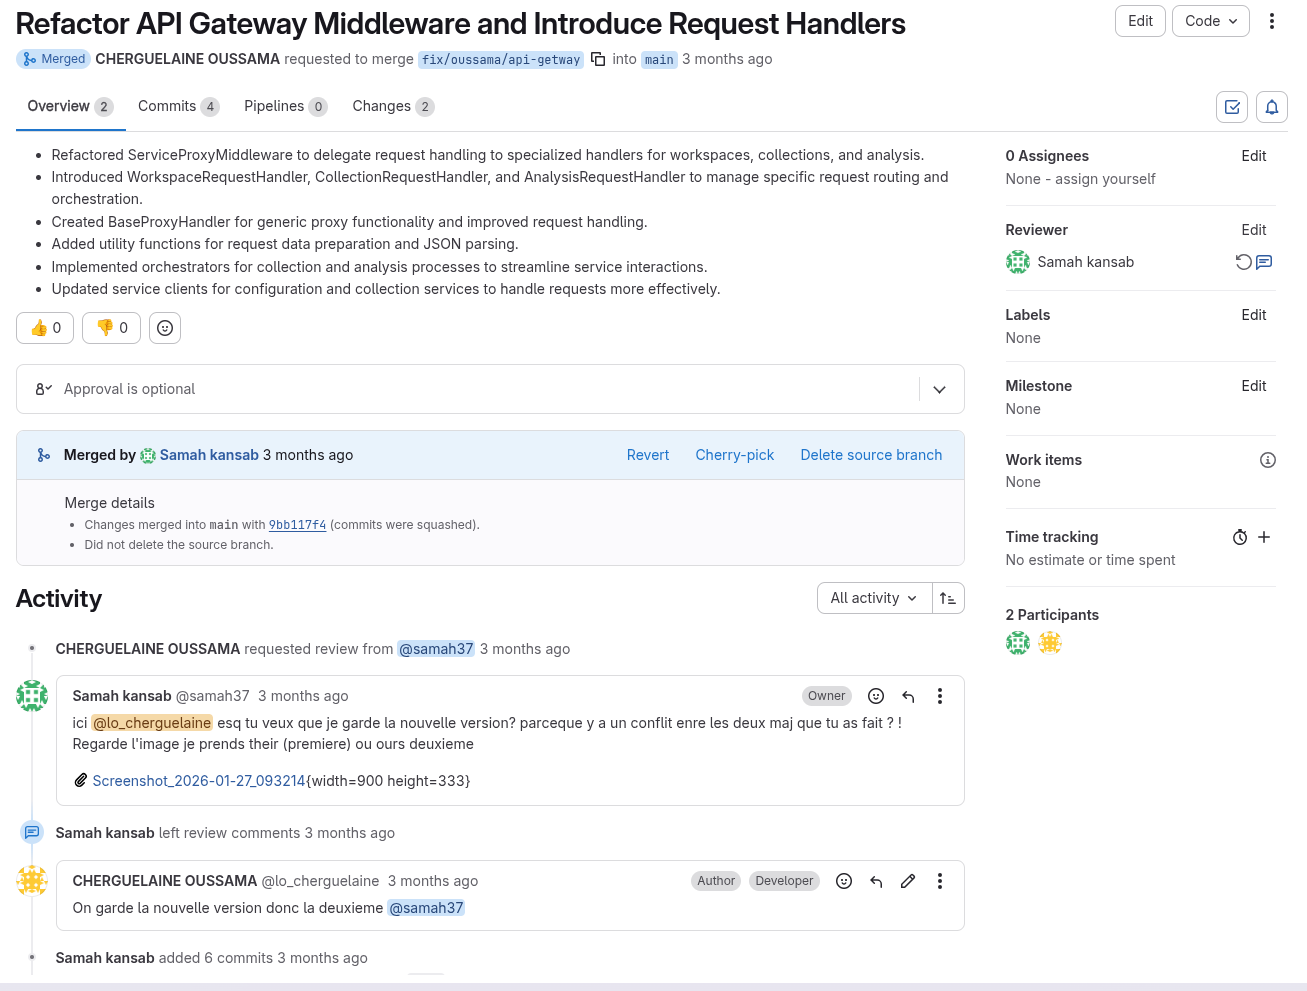
\includegraphics[width=0.95\textwidth]{captures/code_review.png}
    \caption{Exemple de revue de code sur une Merge Request GitLab dans le projet RevMine}
    \label{fig:code-review}
\end{figure}


% ============================================================
\section{Environnement de développement}
% ============================================================

\subsection{Matériel}

Le développement de RevMine a été mené en binôme sur deux postes de travail locaux. Le
Tableau~\ref{tab:env-dev} récapitule leurs configurations matérielles et logicielles.

\begin{table}[H]
\centering
\small
\caption{Configurations des postes de développement}
\label{tab:env-dev}
\begin{tabular}{|>{\raggedright\arraybackslash}p{3.5cm}
                |>{\raggedright\arraybackslash}p{5cm}
                |>{\raggedright\arraybackslash}p{5cm}|}
\hline
\textbf{Caractéristique} & \textbf{Poste 1} & \textbf{Poste 2} \\
\hline
Système d'exploitation & Windows 11 Pro (64~bits) & Windows 11 Pro (64~bits) \\
\hline
Processeur & Intel Core i5 -- 10\textsuperscript{e} génération
           & Intel Core i7 -- 10\textsuperscript{e} génération \\
\hline
Carte graphique & NVIDIA GeForce GTX~1650 & -- \\
\hline
Mémoire RAM & 8~Go & 16~Go \\
\hline
Stockage & SSD 256~Go & SSD 512~Go \\
\hline
\end{tabular}
\end{table}

\subsection{Logiciels et outils}

Les principaux outils utilisés au cours du développement sont les suivants~:

\begin{itemize}
    \item \textbf{Visual Studio Code} et \textbf{PyCharm Community Edition}~: éditeurs utilisés
          respectivement pour le développement frontend/backend généraliste et pour le développement
          Python spécialisé~;
    \item \textbf{Docker Desktop}~: plateforme de conteneurisation permettant d'exécuter et
          d'orchestrer l'ensemble des services sous Windows~;
    \item \textbf{Postman}~: outil de test et de documentation des API REST~;
    \item \textbf{Git / GitLab}~: système de gestion de versions distribué, utilisé pour le
          versioning, la gestion des branches et le suivi du projet~;
    \item \textbf{pgAdmin 4}~: interface graphique d'administration des bases de données
          PostgreSQL.
\end{itemize}

% ============================================================
\section{Technologies utilisées}
% ============================================================

\subsection{Python}
\begin{wrapfigure}{r}{0.1\textwidth}
    \centering
    
\includegraphics[width=0.1\textwidth]{assets/python_logo.png}
\end{wrapfigure}

Python est un langage de programmation interprété, multiparadigme et open source, reconnu pour
sa lisibilité, sa flexibilité et la richesse de son écosystème \parencite{pythonWhatPython}. Sa
syntaxe épurée réduit le coût de maintenance des projets, tandis que ses bibliothèques spécialisées
couvrent de nombreux domaines, de l'analyse de données à l'apprentissage automatique. Dans
RevMine, Python constitue le socle du développement backend en raison de sa maturité pour
l'interaction avec les API REST, le traitement de données et l'intégration de services
d'intelligence artificielle.

\subsection{Django et Django REST Framework}
\begin{wrapfigure}{r}{0.1\textwidth}
    \centering
    
\includegraphics[width=0.1\textwidth]{assets/django_logo.png}
\end{wrapfigure}

Django est un framework web Python suivant le paradigme Modèle-Vue-Template (MVT). Il intègre
nativement un ORM\footnote{ORM (\textit{Object-Relational Mapping})~: technique de correspondance
entre les objets d'un programme et les tables d'une base de données relationnelle, permettant de
manipuler les données sans écrire de requêtes SQL.} puissant, un système d'authentification
robuste et une interface d'administration \parencite{holovaty2009django}. Son extension Django
REST Framework (DRF) facilite la conception d'API RESTful performantes et bien documentées. Ce
framework a été retenu pour les services nécessitant une gestion complexe des données métier --
notamment le service de passerelle d'API, le service de configuration, le service de collecte et
le service d'analyse -- en raison de son architecture modulaire, de son ORM adapté à PostgreSQL
et de ses mécanismes de sécurité intégrés.

\subsection{FastAPI}
\begin{wrapfigure}{r}{0.1\textwidth}
    \centering
    
\includegraphics[width=0.1\textwidth]{assets/fastapi_logo.png}
\end{wrapfigure}

FastAPI est un framework Python moderne orienté performances, reposant sur les annotations de
type Python~3.7+ et le paradigme asynchrone (\texttt{async/await}) \parencite{ramirez2021fastapi}.
Il génère automatiquement une documentation interactive (Swagger UI, ReDoc) et assure la
validation des données via Pydantic. Sa légèreté et sa réactivité native en font un choix adapté
au service LLM de RevMine, pour lequel la rapidité de réponse et la simplicité de l'interface
sont prioritaires.

\subsection{Go et WebSocket}
\begin{wrapfigure}{r}{0.1\textwidth}
    \centering
    
\includegraphics[width=0.1\textwidth]{assets/go_logo.png}
\end{wrapfigure}

Go est un langage compilé et statiquement typé, développé par Google, dont la gestion native de
la concurrence via les \textit{goroutines} en fait un choix de référence pour les services à haute
concurrence et faible latence \parencite{go2012donovan}. Le service de notification de RevMine
doit gérer simultanément un grand nombre de connexions persistantes en temps réel~; Go répond à
cette contrainte en permettant le traitement de milliers de connexions concurrentes avec une
empreinte mémoire réduite. Le framework \textbf{Fiber}, inspiré d'Express.js, a été utilisé pour
simplifier le développement des API REST associées.

Le protocole \textbf{WebSocket}\footnote{WebSocket (RFC~6455)~: protocole de communication
standardisé établissant un canal bidirectionnel et persistant entre un client et un serveur sur
une connexion TCP, contrairement à HTTP qui est unidirectionnel par nature.} établit un canal de
communication bidirectionnel et persistant, permettant au service de notification de diffuser
instantanément les événements système (démarrage de collecte, fin d'analyse, erreur) aux clients
connectés, sans recourir au \textit{polling} HTTP.

\subsection{React.js}
\begin{wrapfigure}{r}{0.1\textwidth}
    \centering
    
\includegraphics[width=0.1\textwidth]{assets/react_logo.png}
\end{wrapfigure}

React.js est une bibliothèque JavaScript open source développée par Meta pour la construction
d'interfaces utilisateur interactives, reposant sur une architecture en composants réutilisables
et une gestion efficace du DOM virtuel \parencite{facebookReact2023}. Dans RevMine, React.js
assure le développement de l'interface utilisateur, permettant l'exploration interactive des
données, la configuration des collectes et la visualisation des résultats d'analyse.

\subsection{Tailwind CSS}
\begin{wrapfigure}{r}{0.1\textwidth}
    \centering
    
\includegraphics[width=0.1\textwidth]{assets/tailwind_logo.png}
\end{wrapfigure}

Tailwind CSS est un framework CSS \textit{utility-first} qui permet de construire des interfaces
modernes et responsives directement dans le balisage, sans rédiger de feuilles de style
personnalisées volumineuses \parencite{tailwindlabs2023}. Son approche par classes utilitaires
composables favorise la cohérence visuelle et s'intègre naturellement avec React.

\subsection{Docker}
\begin{wrapfigure}{r}{0.1\textwidth}
    \centering
    
\includegraphics[width=0.1\textwidth]{assets/docker_logo.png}
\end{wrapfigure}

Docker est une plateforme de conteneurisation permettant d'empaqueter une application et ses
dépendances dans un conteneur léger, portable et isolé \parencite{merkel2014docker}. Un
\textit{conteneur} est une unité d'exécution autonome qui encapsule le code, les bibliothèques
et les configurations nécessaires au fonctionnement d'un service, garantissant ainsi un
comportement identique quel que soit l'environnement d'exécution. Docker Compose étend cette
capacité en orchestrant plusieurs services applicatifs et d'infrastructure de manière
déclarative. Dans RevMine, Docker assure la conteneurisation de l'ensemble des services,
garantissant la reproductibilité des environnements entre le développement, les tests et le
déploiement.

\subsection{PostgreSQL}
\begin{wrapfigure}{r}{0.1\textwidth}
    \centering
    
\includegraphics[width=0.1\textwidth]{assets/postgresql_logo.png}
\end{wrapfigure}

PostgreSQL est un système de gestion de base de données relationnelle objet open source, reconnu
pour sa robustesse, sa conformité aux standards SQL et ses fonctionnalités avancées
\parencite{postgresql2023}. Son intégration native avec l'ORM Django facilite la persistance des
données métier. Chaque microservice de RevMine dispose de sa propre base PostgreSQL, assurant
ainsi l'isolation des données et limitant les dépendances directes entre services.

\subsection{MinIO}
\begin{wrapfigure}{r}{0.1\textwidth}
    \centering
    
\includegraphics[width=0.1\textwidth]{assets/minio_logo.png}
\end{wrapfigure}

MinIO est une solution de stockage objet haute performance compatible avec l'API Amazon S3,
conçue pour le stockage de fichiers volumineux et de données semi-structurées
\parencite{minio2023}. Dans RevMine, MinIO archive les données brutes collectées depuis GitHub et
GitLab sous forme de fichiers JSON, séparant ainsi les artefacts bruts du stockage relationnel et
facilitant leur réutilisation sans relancer les appels API.

\subsection{Apache Kafka}
\begin{wrapfigure}{r}{0.1\textwidth}
    \centering
    
\includegraphics[width=0.1\textwidth]{assets/kafka_logo.png}
\end{wrapfigure}

Apache Kafka est une plateforme distribuée de \textit{streaming} d'événements permettant la
communication asynchrone entre services via un mécanisme de publication/souscription
(\textit{publish/subscribe}) \parencite{kreps2011kafka}. Dans ce modèle, un service
\textit{producteur} publie des messages sur un \textit{topic} -- canal logique nommé --, et un ou
plusieurs services \textit{consommateurs} s'abonnent à ce topic pour traiter les messages de
manière indépendante. Son adoption dans RevMine réduit le couplage entre microservices, améliore
la scalabilité du système et permet l'exécution de traitements indépendants ou différés.

\subsection{Redis et Celery}
\begin{wrapfigure}{r}{0.1\textwidth}
    \centering
    
\includegraphics[width=0.1\textwidth]{assets/redis_logo.png}
\end{wrapfigure}

Redis est un système de stockage clé-valeur en mémoire offrant de très hautes performances pour
la mise en cache et la récupération rapide de données \parencite{carlson2013redis}. Dans RevMine,
Redis remplit deux rôles complémentaires~: le cache applicatif, qui réduit le nombre de requêtes
répétitives vers les bases de données, et le broker de messages pour Celery.

Celery est un gestionnaire de tâches asynchrones pour Python qui permet d'exécuter des
traitements longs en arrière-plan, sans bloquer la réponse aux requêtes HTTP. Cette combinaison
Redis~+~Celery améliore la réactivité globale de la plateforme, notamment lors de l'analyse de
jeux de données volumineux.

\subsection{Pile d'observabilité~: Grafana, Loki et Promtail}
\label{subsec:observabilite}
\begin{wrapfigure}{r}{0.1\textwidth}
    \centering
    
\includegraphics[width=0.1\textwidth]{assets/grafana_logo.png}
\end{wrapfigure}

La supervision des journaux applicatifs repose sur la pile \textbf{Loki + Promtail + Grafana}
\parencite{grafana2023loki}. Cette solution a été préférée à des alternatives plus lourdes
(ELK Stack) en raison de sa faible empreinte mémoire et de son intégration native dans un
environnement Docker.

\begin{itemize}
    \item \textbf{Promtail}~: agent déployé en tant que conteneur Docker, il collecte les journaux
          de sortie standard (\texttt{stdout}/\texttt{stderr}) de chaque conteneur applicatif et les
          expédie vers Loki~;
    \item \textbf{Loki}~: moteur de stockage et d'indexation des journaux, optimisé pour les
          environnements conteneurisés. Contrairement à Elasticsearch, Loki n'indexe que les
          métadonnées (labels), ce qui réduit considérablement la consommation de ressources~;
    \item \textbf{Grafana}~: interface de visualisation permettant d'interroger Loki via le langage
          de requête LogQL, d'afficher les journaux en temps réel et de configurer des alertes.
\end{itemize}

Dans RevMine, chaque service produit ses journaux en JSON structuré, permettant à Grafana de
filtrer rapidement les erreurs et d'identifier les anomalies par service, par niveau de sévérité
ou par période.

\subsection{SonarQube}
\label{subsec:sonarqube-tech}
\begin{wrapfigure}{r}{0.1\textwidth}
    \centering
    
\includegraphics[width=0.1\textwidth]{assets/sonarqube_logo.png}
\end{wrapfigure}

SonarQube est une plateforme d'analyse statique de la qualité du code, capable de détecter des
bugs, des vulnérabilités de sécurité, des \textit{code smells} et des duplications
\parencite{campbell2013sonarqube}. Dans RevMine, SonarQube Community~10.4 est déployé comme
conteneur Docker et intégré directement dans le pipeline GitLab CI. Un \textbf{Quality Gate}
bloquant a été configuré~: si les seuils de qualité ne sont pas atteints, le pipeline est
interrompu avant l'étape de build, garantissant qu'aucun code dégradé ne passe en intégration.

% ============================================================
\section{Réalisation du backend}
% ============================================================

Le backend de RevMine est composé de plusieurs microservices spécialisés, chacun prenant en
charge un périmètre fonctionnel précis. Les sections suivantes détaillent l'implémentation de
chacun d'eux.

% ------------------------------------------------------------
\subsection{Service de passerelle d'API}
% ------------------------------------------------------------

Le service de passerelle d'API (\textit{API Gateway}) constitue le point d'entrée unique de
l'application. Développé avec \textbf{Django} et \textbf{Django REST Framework}, il centralise
l'authentification des utilisateurs et orchestre les appels vers les services internes, évitant
ainsi au frontend d'avoir à connaître l'adresse de chaque microservice.

Ce service gère l'inscription, la connexion et la gestion du profil utilisateur. L'authentification
repose sur des \textbf{tokens JWT}\footnote{JWT (\textit{JSON Web Token})~: standard ouvert (RFC
7519) définissant un format compact et autonome pour la transmission sécurisée d'informations entre
parties sous forme d'objet JSON signé numériquement.}, avec prise en charge du rafraîchissement
de session par l'émission d'un \textit{refresh token} de longue durée. En complément de
l'authentification classique par email et mot de passe, le service intègre l'authentification
\textbf{OAuth}\footnote{OAuth (\textit{Open Authorization})~: protocole standard d'autorisation
permettant à une application d'accéder aux ressources d'un utilisateur chez un fournisseur tiers
sans que l'utilisateur n'ait à partager ses identifiants.} via GitHub, GitLab et Google,
simplifiant l'accès à la plateforme pour les développeurs.

La documentation interactive des API est générée automatiquement grâce à
\textbf{drf-spectacular}. Les principaux endpoints exposés par ce service sont détaillés dans
le tableau ci-après.

\begin{table}[H]
\centering
\small
\caption{Endpoints principaux du service de passerelle d'API}
\label{tab:endpoints-gateway}
\begin{tabular}{|>{\centering\arraybackslash}p{1.6cm}
                |>{\raggedright\arraybackslash}p{6.2cm}
                |>{\raggedright\arraybackslash}p{4.8cm}|}
\hline
\textbf{Méthode} & \textbf{Route} & \textbf{Description} \\
\hline
POST & \texttt{/api/auth/register} & Inscription d'un nouvel utilisateur \\
\hline
POST & \texttt{/api/auth/login} & Authentification par email et mot de passe \\
\hline
POST & \texttt{/api/auth/refresh} & Renouvellement du token JWT \\
\hline
GET & \texttt{/api/auth/me} & Profil de l'utilisateur connecté \\
\hline
PATCH & \texttt{/api/auth/me/update/} & Mise à jour des informations du profil \\
\hline
POST & \texttt{/api/auth/me/change-password/} & Changement de mot de passe \\
\hline
DELETE & \texttt{/api/auth/me/delete/} & Suppression du compte utilisateur \\
\hline
GET / POST & \texttt{/api/auth/oauth/github} & Authentification OAuth via GitHub \\
\hline
GET / POST & \texttt{/api/auth/oauth/gitlab} & Authentification OAuth via GitLab \\
\hline
GET / POST & \texttt{/api/auth/oauth/google} & Authentification OAuth via Google \\
\hline
GET & \texttt{/api/docs/} & Documentation Swagger interactive \\
\hline
\end{tabular}
\end{table}

% ------------------------------------------------------------
\subsection{Service de configuration}
% ------------------------------------------------------------

Le service de configuration gère les \textit{workspaces} et les dépôts associés. Il permet à
l'utilisateur de créer un espace de travail, de spécifier la plateforme cible (GitHub ou GitLab),
de fournir un jeton d'accès\footnote{Un jeton d'accès (\textit{access token}) est une clé secrète
générée par une plateforme permettant à une application tierce d'interagir avec son API au nom de
l'utilisateur, sans exposer les identifiants de connexion.} et de valider la connexion. Une fois
la connexion établie, le service interroge la plateforme distante pour récupérer la liste des
dépôts disponibles, que l'utilisateur peut ensuite importer dans son espace local.

La séparation entre la gestion des sources de données et les traitements analytiques améliore la
maintenabilité de l'ensemble et facilite l'évolution indépendante de chaque composant. Les
endpoints de ce service sont répertoriés dans le tableau suivant.

\begin{table}[H]
\centering
\small
\caption{Endpoints principaux du service de configuration}
\label{tab:endpoints-config}
\begin{tabular}{|>{\centering\arraybackslash}p{2cm}
                |>{\raggedright\arraybackslash}p{7cm}
                |>{\raggedright\arraybackslash}p{3.5cm}|}
\hline
\textbf{Méthode} & \textbf{Route} & \textbf{Description} \\
\hline
GET / POST & \texttt{/api/workspaces/} & Liste et création de workspaces \\
\hline
GET / PUT / DELETE & \texttt{/api/workspaces/<id>/} & Lecture, mise à jour, suppression \\
\hline
GET & \texttt{/api/workspaces/<id>/token/} & Récupération du token chiffré \\
\hline
POST & \texttt{/api/workspaces/test/} & Test de connexion à la plateforme \\
\hline
GET & \makecell[l]{\texttt{/api/workspaces/<id>/} \\ \texttt{remote-repositories/}} & Dépôts distants disponibles \\
\hline
POST & \makecell[l]{\texttt{/api/workspaces/<id>/} \\ \texttt{repositories/import/}} & Import local des dépôts sélectionnés \\
\hline
GET & \texttt{/api/workspaces/<id>/repositories/} & Liste des dépôts importés \\
\hline
DELETE & \makecell[l]{\texttt{/api/workspaces/<id>/} \\ \texttt{repositories/<repo\_id>/}} & Suppression d'un dépôt importé \\
\hline
GET & \texttt{/api/workspaces/repositories/all/} & Liste globale de tous les dépôts \\
\hline
\end{tabular}
\end{table}

% ------------------------------------------------------------
\subsection{Service de collecte}
% ------------------------------------------------------------

Le service de collecte est l'un des modules centraux de RevMine. Il récupère les données issues
des plateformes de développement -- notamment les \textit{merge requests}, \textit{pull requests},
branches et métadonnées associées depuis GitHub et GitLab -- selon un \textbf{workflow progressif}
structuré en six étapes~:

\begin{enumerate}
    \item sélection du dépôt à traiter~;
    \item récupération des branches disponibles~;
    \item sélection des métriques à collecter~;
    \item validation du plan de collecte~;
    \item exécution, suspension ou reprise de la collecte~;
    \item consultation des résultats.
\end{enumerate}

Ce service prend également en charge l'\textbf{importation de collections externes} au format
JSON, permettant d'intégrer des données déjà exportées depuis d'autres sources. Les données brutes
collectées sont archivées dans \textbf{MinIO}, tandis que les métadonnées de suivi sont conservées
en base relationnelle.

Une étape de \textbf{nettoyage et de structuration} transforme ensuite les données brutes en
fichiers CSV exploitables, prêts pour l'analyse. Cette séparation entre collecte et préparation
des données garantit la traçabilité et facilite la réutilisation des jeux de données. Le tableau
ci-dessous liste les endpoints exposés par ce service.

\begin{table}[H]
\centering
\small
\caption{Endpoints principaux du service de collecte}
\label{tab:endpoints-collection}
\begin{tabular}{|>{\centering\arraybackslash}p{1.5cm}
                |>{\raggedright\arraybackslash}p{7.2cm}
                |>{\raggedright\arraybackslash}p{3.8cm}|}
\hline
\textbf{Méthode} & \textbf{Route} & \textbf{Description} \\
\hline
POST & \texttt{/api/collections/start/} & Initialisation d'un plan de collecte \\
\hline
POST & \makecell[l]{\texttt{/api/collections/plans/<id>/} \\ \texttt{configure/}} & Sélection des métriques \\
\hline
POST & \makecell[l]{\texttt{/api/collections/plans/<id>/} \\ \texttt{validate/}} & Validation du plan de collecte \\
\hline
POST & \makecell[l]{\texttt{/api/collections/plans/<id>/} \\ \texttt{execute/}} & Lancement de la collecte \\
\hline
GET & \makecell[l]{\texttt{/api/collections/plans/<id>/} \\ \texttt{status/}} & Suivi de la progression \\
\hline
POST & \makecell[l]{\texttt{/api/collections/plans/<id>/} \\ \texttt{pause/}} & Suspension de la collecte \\
\hline
POST & \makecell[l]{\texttt{/api/collections/plans/<id>/} \\ \texttt{resume/}} & Reprise d'une collecte suspendue \\
\hline
POST & \makecell[l]{\texttt{/api/collections/plans/<id>/} \\ \texttt{apply-filters/}} & Filtres et génération du CSV \\
\hline
GET & \makecell[l]{\texttt{/api/collections/cleaned-data/} \\ \texttt{<id>/download/<type>/}} & Téléchargement du CSV généré \\
\hline
POST & \texttt{/api/collections/upload-external/} & Import d'une collection externe \\
\hline
\end{tabular}
\end{table}

% ------------------------------------------------------------
\subsection{Service d'analyse}
% ------------------------------------------------------------

Le service d'analyse transforme les datasets préparés en résultats analytiques et visuels. Il
permet d'importer des datasets, d'afficher un aperçu des colonnes disponibles, d'identifier
automatiquement les métriques compatibles et de générer des graphiques correspondants.

Pour gérer les traitements potentiellement coûteux en temps, le service s'appuie sur
\textbf{Celery} pour l'exécution asynchrone des tâches et sur \textbf{Redis} comme broker de
messages. Cette architecture permet à l'interface utilisateur de rester réactive pendant
l'exécution des calculs, notamment lors de l'analyse de jeux de données volumineux ou de la
génération de plusieurs visualisations en parallèle. Les analyses réalisées sont sauvegardées
et consultables via un historique. Le cycle de vie complet d'une analyse est couvert par les
endpoints répertoriés dans le tableau suivant.

\begin{table}[H]
\centering
\small
\caption{Endpoints principaux du service d'analyse}
\label{tab:endpoints-analyze}
\begin{tabular}{|>{\centering\arraybackslash}p{1.5cm}
                |>{\raggedright\arraybackslash}p{7.2cm}
                |>{\raggedright\arraybackslash}p{3.8cm}|}
\hline
\textbf{Méthode} & \textbf{Route} & \textbf{Description} \\
\hline
POST & \texttt{/api/analysis/datasets/upload/} & Import d'un dataset (CSV) \\
\hline
GET & \texttt{/api/analysis/datasets/<id>/columns/} & Colonnes et types disponibles \\
\hline
GET & \texttt{/api/analysis/datasets/<id>/preview/} & Aperçu des premières lignes \\
\hline
GET & \makecell[l]{\texttt{/api/analysis/datasets/<id>/} \\ \texttt{available\_metrics/}} & Métriques compatibles \\
\hline
POST & \texttt{/api/analysis/generate/} & Génération d'un graphique \\
\hline
GET & \texttt{/api/analysis/analyses/} & Historique des analyses réalisées \\
\hline
POST & \texttt{/api/analysis/analyses/bulk\_create/} & Création de plusieurs analyses \\
\hline
GET & \texttt{/api/analysis/analyses/<id>/result/} & Résultat et image du graphique \\
\hline
POST & \texttt{/api/analysis/analyses/<id>/retry/} & Relance d'une analyse existante \\
\hline
GET & \texttt{/api/analysis/metrics/} & Catalogue des métriques disponibles \\
\hline
\end{tabular}
\end{table}

% ------------------------------------------------------------
\subsection{Service d'intelligence artificielle}
% ------------------------------------------------------------

RevMine intègre un service dédié au traitement du langage naturel (NLP/LLM\footnote{LLM
(\textit{Large Language Model})~: modèle de langage de grande taille, entraîné sur de vastes
corpus textuels, capable de comprendre et de générer du texte en langage naturel.}), développé
avec \textbf{FastAPI}. Ce service constitue l'interface entre l'utilisateur et les modèles de
langage~: il interprète des requêtes formulées en langage naturel -- telles que \og{}Analyse les
données des six derniers mois sur la branche principale\fg{} -- et les transforme en paramètres
structurés exploitables par les autres services.

\subsubsection*{Ingénierie des prompts}

Le c\oe{}ur du service repose sur une ingénierie de prompts\footnote{\textit{Prompt engineering}~:
discipline consistant à concevoir et structurer les instructions transmises à un modèle de langage
afin de maximiser la pertinence, la fiabilité et la conformité de ses réponses.} structurée,
élaborée selon un processus de consensus en quatre étapes inspiré de la \textit{Nominal Group
Technique} (NGT). Cette démarche vise à justifier chaque instruction du prompt par un mode de
défaillance concret identifié à partir du mode de configuration manuelle~: hallucination de
métriques, omission de dépendances, mauvaise détection de la plateforme, résolution incorrecte
des expressions temporelles, JSON malformé.

Chaque requête envoyée au modèle se compose de deux parties~:
\begin{itemize}
    \item un \textbf{prompt système}, qui définit le rôle du modèle, le format de sortie attendu
          (JSON strict) et l'ensemble des contraintes opérationnelles~: métriques valides,
          dépendances, indicateurs de plateforme, règles de filtres et ancrage temporel~;
    \item un \textbf{prompt utilisateur}, qui contient la requête en langage naturel saisie.
\end{itemize}

Le processus d'élaboration s'est déroulé en quatre étapes successives~: (1)~\textbf{élicitation
indépendante} -- chaque auteur du binôme identifie les éléments nécessaires à partir du schéma
opérationnel de RevMine~; (2)~\textbf{consolidation structurée} -- seuls les éléments liés à un
mode de défaillance concret sont retenus~; (3)~\textbf{construction et vérification interne} par
l'autre auteur~; (4)~\textbf{validation croisée} par le binôme. Sept éléments fondamentaux ont
ainsi été intégrés au prompt, résumés dans le Tableau~\ref{tab:prompt_elements_fr}.

\begin{table}[H]
\centering
\small
\caption{Éléments du prompt système et modes de défaillance prévenus}
\label{tab:prompt_elements_fr}
\begin{tabular}{|>{\raggedright\arraybackslash}p{6.5cm}
                |>{\raggedright\arraybackslash}p{6.5cm}|}
\hline
\textbf{Élément du prompt} & \textbf{Mode de défaillance prévenu} \\
\hline
Énumération fermée de toutes les métriques valides & Hallucination de noms de métriques \\
\hline
Table de dépendances métriques\,/\,features & Omission de dépendances \\
\hline
Règles de classification de l'intention & Mauvaise classification de l'intention \\
\hline
Indicateurs de détection de la plateforme & Confusion GitHub\,/\,GitLab \\
\hline
Injection dynamique de la date courante (\texttt{\_\_TODAY\_\_}) & Mauvaise résolution des expressions temporelles \\
\hline
Règles de peuplement des filtres & Filtres incorrects ou manquants \\
\hline
Instruction de discipline de sortie stricte & JSON mal formé ou encadré de texte \\
\hline
\end{tabular}
\end{table}

Le modèle est instruit de répondre exclusivement en JSON valide, sans texte explicatif, permettant
au backend de désérialiser directement la réponse.

\subsubsection*{Mode Ollama -- inférence locale}

Ollama est un moteur d'inférence locale permettant d'exécuter des modèles open source (Mistral,
LLaMA, Gemma, etc.) directement sur la machine hôte, sans dépendance à un service cloud
\parencite{ollama2023}. Ce mode garantit la confidentialité totale des données et l'absence de
coût par requête, au prix de performances limitées par les ressources locales disponibles.

\subsubsection*{Mode OpenRouter -- modèles hébergés}

OpenRouter est une passerelle d'API agrégeant de nombreux fournisseurs de LLM (OpenAI, Anthropic,
Google, Meta, etc.) sous une interface unifiée compatible avec l'API OpenAI
\parencite{openrouter2023}. Ce mode donne accès à des modèles de grande capacité sans
infrastructure GPU requise, avec une flexibilité selon le budget et la tâche, au prix d'une
dépendance à un service externe.

L'utilisateur peut choisir le mode selon ses contraintes de confidentialité, de coût et de
qualité. L'architecture indépendante du service LLM permet de le faire évoluer sans impact sur
les autres services. Les endpoints exposés par ce service sont les suivants~:

\begin{table}[H]
\centering
\small
\caption{Endpoints du service LLM (FastAPI)}
\label{tab:endpoints-llm}
\begin{tabular}{|>{\centering\arraybackslash}p{1.5cm}
                |>{\raggedright\arraybackslash}p{4.5cm}
                |>{\raggedright\arraybackslash}p{6.5cm}|}
\hline
\textbf{Méthode} & \textbf{Route} & \textbf{Description} \\
\hline
GET & \texttt{/health} & Vérification de l'état du service \\
\hline
GET & \texttt{/models} & Liste des fournisseurs et modèles disponibles \\
\hline
POST & \texttt{/ollama} & Traitement via Ollama (inférence locale) \\
\hline
POST & \texttt{/openrouter} & Traitement via OpenRouter (hébergé) \\
\hline
\end{tabular}
\end{table}

% ------------------------------------------------------------
\subsection{Service de notification}
% ------------------------------------------------------------

Le service de notification a été développé en \textbf{Go} avec le framework \textbf{Fiber}. Ce
choix répond à la nécessité de gérer un grand nombre de connexions WebSocket concurrentes avec
une faible empreinte mémoire, exigence difficile à satisfaire avec des frameworks synchrones
traditionnels.

Ce service consomme les événements publiés sur Kafka par les autres services, les persiste dans
sa propre base PostgreSQL, puis les diffuse en temps réel aux clients connectés via WebSocket.
L'utilisateur reçoit ainsi instantanément des informations sur l'état d'une collecte, la fin
d'un traitement ou toute anomalie survenue. Des endpoints complémentaires permettent de lister
les notifications, de comptabiliser les éléments non lus, de les marquer comme lus ou de les
supprimer.

% ============================================================
\section{Gestion des données et communication inter-services}
% ============================================================

La cohérence globale de RevMine repose sur une stratégie claire de gestion des données. Chaque
microservice dispose de sa propre base \textbf{PostgreSQL}, garantissant l'isolation des
responsabilités et limitant les dépendances directes entre services -- principe fondateur de
l'architecture microservices.

Les données brutes issues de la collecte sont archivées dans \textbf{MinIO} au format JSON,
séparant ainsi les artefacts bruts du stockage relationnel et facilitant leur réutilisation sans
relancer les appels API vers les plateformes distantes.

La communication entre services s'articule autour de deux mécanismes complémentaires~:

\begin{itemize}
    \item les \textbf{API REST}, pour les interactions synchrones initiées par le frontend ou le
          service de passerelle d'API, lorsqu'une réponse immédiate est attendue~;
    \item \textbf{Apache Kafka}, comme bus de messages pour la communication asynchrone et le
          découplage des traitements internes, notamment pour les opérations longues telles que
          la collecte ou l'analyse de données.
\end{itemize}

Ces topics permettent, par exemple, au service de collecte d'informer le service d'analyse et
le service de notification de la disponibilité de nouvelles données, sans aucun couplage direct
entre eux. Le Tableau~\ref{tab:kafka-topics} détaille les topics Kafka utilisés dans la
plateforme, ainsi que leurs producteurs et consommateurs respectifs.

\begin{table}[H]
\centering
\small
\caption{Topics Kafka et flux de messages dans RevMine}
\label{tab:kafka-topics}
\begin{tabular}{|>{\raggedright\arraybackslash}p{6.2cm}
                |>{\raggedright\arraybackslash}p{3cm}
                |>{\raggedright\arraybackslash}p{3.5cm}|}
\hline
\textbf{Topic} & \textbf{Producteur} & \textbf{Consommateur(s)} \\
\hline
\texttt{config.tokens.request} & Collecte / Analyse & Configuration \\
\hline
\texttt{config.tokens.response} & Configuration & Collecte / Analyse \\
\hline
\texttt{collection.events.started} & Collecte & Notification \\
\hline
\texttt{collection.events.completed} & Collecte & Analyse, Notification \\
\hline
\texttt{collection.events.failed} & Collecte & Notification \\
\hline
\texttt{analysis.events.requested} & Analyse & Analyse \\
\hline
\texttt{analysis.events.completed} & Analyse & Notification \\
\hline
\texttt{notification.events} & Tous les services & Notification \\
\hline
\end{tabular}
\end{table}

% ============================================================
\section{Réalisation du frontend}
% ============================================================

Le frontend de RevMine a été développé sous la forme d'une \textbf{Single Page Application}
(SPA)\footnote{SPA (\textit{Single Page Application})~: application web qui charge une seule
page HTML au démarrage et met à jour dynamiquement le contenu sans rechargement complet de la
page, offrant une expérience utilisateur proche d'une application native.} avec \textbf{React},
offrant une navigation fluide entre les fonctionnalités.

\subsection{Structure générale de l'interface}

La navigation est assurée par \textbf{React Router} et les vues sont organisées en pages
fonctionnelles~: authentification, gestion des workspaces, gestion des projets, collecte et
nettoyage des données, analyse, profil et paramètres. Des \textit{layouts} distincts délimitent
les espaces accessibles sans authentification et les pages réservées aux utilisateurs connectés.

\subsection{Gestion de l'authentification et de l'état global}

L'authentification est centralisée dans des \textit{providers} React. Lors de la connexion, les
tokens JWT sont stockés côté client et automatiquement injectés dans les en-têtes des requêtes
HTTP via des \textbf{intercepteurs Axios}. Un mécanisme de rafraîchissement silencieux évite toute
interruption de session en cas d'expiration du token d'accès. La protection des routes garantit
que les pages sensibles sont inaccessibles aux utilisateurs non authentifiés.

\subsection{Modules fonctionnels}

\paragraph{Gestion des workspaces et des projets.} Ce module permet à l'utilisateur de créer et
gérer ses espaces de travail, de tester la connexion à une plateforme distante et d'importer les
dépôts souhaités. L'organisation par workspace puis par dépôt reflète le processus naturel de
travail dans un environnement de développement collaboratif.

\paragraph{Collecte et nettoyage des données.} L'interface de collecte guide l'utilisateur à
travers les étapes de configuration du plan de collecte~: sélection des branches, des métriques
et des filtres. Des écrans dédiés permettent de suivre la progression de l'exécution et de
consulter les résultats. Une fois les données récupérées, des vues spécifiques donnent accès au
nettoyage, à la génération de fichiers CSV structurés et à la consultation des jeux de données
préparés.

\paragraph{Analyse et visualisation.} Le module d'analyse constitue l'une des fonctionnalités
centrales de RevMine. Il permet de lancer une analyse à partir d'un fichier CSV ou d'un dataset
préparé, de sélectionner les métriques disponibles et de générer des représentations graphiques
adaptées au contenu des données. L'interface propose également un historique des analyses et un
tableau de bord analytique. Les visualisations sont produites avec \textbf{ECharts}, une
bibliothèque graphique offrant des représentations riches et interactives.

\subsection{Aspects ergonomiques et visuels}

L'interface repose sur \textbf{Tailwind CSS}, qui assure la cohérence des composants, des
espacements et des couleurs, tout en garantissant un comportement adaptatif sur différentes
tailles d'écran. L'organisation modulaire des composants React et l'utilisation de contextes
partagés contribuent à la maintenabilité du code frontend.

% ============================================================
\section{Sécurité de la solution}
% ============================================================

La sécurité a été intégrée dès la phase de conception, selon le principe du
\textit{security by design}. L'accès aux fonctionnalités sensibles est protégé par une
authentification fondée sur \textbf{JWT}. Les routes privées du frontend sont filtrées côté
client, tandis que les endpoints backend exigent un token d'accès valide pour l'ensemble des
opérations métier.

Les tokens d'accès aux plateformes tierces sont stockés de manière chiffrée en base de données
-- en utilisant l'algorithme symétrique AES via la bibliothèque Fernet -- limitant les risques
en cas de compromission. L'intégration de l'authentification \textbf{OAuth} délègue la gestion
de l'identité à des fournisseurs de confiance (GitHub, GitLab, Google), améliorant à la fois la
sécurité et l'expérience utilisateur en supprimant la nécessité de créer un nouveau mot de passe.

% ============================================================
\section{Tests et validation}
% ============================================================

\subsection{Stratégie de test}

La stratégie de test adoptée pour RevMine s'articule autour de quatre niveaux complémentaires,
conformément aux bonnes pratiques de l'ingénierie logicielle~:

\begin{itemize}
    \item \textbf{Tests unitaires}~: vérification isolée des fonctions, classes et composants
          individuels au sein de chaque service backend et du frontend~;
    \item \textbf{Tests d'intégration}~: validation des interactions entre les couches d'un même
          service, notamment entre la couche service, la couche domaine et la couche
          infrastructure~;
    \item \textbf{Tests fonctionnels (\textit{end-to-end})}~: simulation de scénarios utilisateur
          complets dans un environnement proche de la production, à l'aide de Cypress~;
    \item \textbf{Tests de non-régression}~: exécutés automatiquement à chaque commit via le
          pipeline GitLab CI, afin de détecter toute régression introduite par les nouvelles
          modifications.
\end{itemize}

Les outils de test mobilisés pour chacune des couches de la plateforme sont récapitulés dans le
Tableau~\ref{tab:outils-tests}.

\begin{table}[H]
\centering
\small
\caption{Outils de test utilisés dans RevMine}
\label{tab:outils-tests}
\begin{tabular}{|>{\raggedright\arraybackslash}p{3.5cm}
                |>{\raggedright\arraybackslash}p{3.8cm}
                |>{\raggedright\arraybackslash}p{5.5cm}|}
\hline
\textbf{Couche} & \textbf{Outil} & \textbf{Périmètre couvert} \\
\hline
Backend Python & pytest + pytest-django & Tests unitaires et d'intégration \\
\hline
Frontend React & Jest + React Testing Library & Tests des services et composants JS \\
\hline
End-to-End & Cypress & Scénarios fonctionnels complets \\
\hline
Qualité statique & SonarQube 10.4 & Couverture, bugs, \textit{code smells} \\
\hline
CI/CD & GitLab CI & Automatisation des tests et build Docker \\
\hline
Couverture & Cobertura (\texttt{coverage.xml}) & Rapports de couverture par service \\
\hline
Service LLM & Benchmark (500~scénarios) & Parsing langage naturel vers JSON conforme \\
\hline
\end{tabular}
\end{table}

% ------------------------------------------------------------
\subsection{Tests unitaires}
% ------------------------------------------------------------

Les tests unitaires constituent le premier niveau de validation. Ils vérifient le comportement
de chaque unité logique indépendamment des autres composants. Dans RevMine, chaque service
backend dispose de son propre dossier de tests, organisé en fichiers thématiques et exécuté via
le framework \textbf{pytest}.

\subsubsection*{Service de passerelle d'API}

Les tests de la passerelle d'API, définis dans le fichier \texttt{test\_pipeline\_robustness.py},
jouent un rôle de sentinelle~: ils vérifient que l'ensemble du pipeline d'intégration continue
fonctionne correctement. L'analyse du rapport de couverture révèle un taux de
\textbf{57,97\,\%}, correspondant à 909~lignes couvertes sur 1\,568~lignes valides.

\subsubsection*{Service de configuration}

Le service de configuration dispose d'une suite de tests complète répartie sur sept fichiers,
organisés selon les couches de l'architecture propre (\textit{clean architecture}) adoptée.
Les différents fichiers de tests et leur périmètre de couverture sont présentés dans le
Tableau~\ref{tab:tests-config}.

\begin{table}[H]
\centering
\small
\caption{Fichiers de tests du service de configuration}
\label{tab:tests-config}
\begin{tabular}{|>{\raggedright\arraybackslash}p{6cm}
                |>{\raggedright\arraybackslash}p{7cm}|}
\hline
\textbf{Fichier de test} & \textbf{Périmètre couvert} \\
\hline
\texttt{test\_api\_views.py} & Endpoints REST (CRUD workspaces et dépôts, test de connexion) \\
\hline
\texttt{test\_encryption.py} & Chiffrement et déchiffrement des tokens AES via Fernet \\
\hline
\texttt{test\_kafka\_handlers.py} & Publication et consommation sur les topics \texttt{config.tokens.*} \\
\hline
\texttt{test\_repository\_service.py} & Récupération et import des dépôts depuis GitHub et GitLab \\
\hline
\texttt{test\_workspace\_rules.py} & Règles métier (unicité du nom, validation de plateforme, URL) \\
\hline
\texttt{test\_workspace\_service.py} & Cycle de vie du workspace (création, test, mise à jour) \\
\hline
\texttt{test\_workspaces.py} & Tests d'intégration des couches combinées (suite héritée) \\
\hline
\end{tabular}
\end{table}

Cette suite totalise \textbf{88~tests}, dont 30~tests hérités et 58~nouveaux tests couvrant
l'architecture refactorisée. La présence de tests dédiés à la couche domaine
(\texttt{test\_workspace\_rules.py}) et à la couche infrastructure (\texttt{test\_encryption.py},
\texttt{test\_kafka\_handlers.py}) traduit une approche rigoureuse de la validation à chaque
niveau de l'architecture.

\subsubsection*{Service de collecte}

Le service de collecte est structuré autour de cinq fichiers de tests thématiques, complétés
d'un fichier de fixtures\footnote{\textit{Fixture}~: en terminologie de test logiciel, ensemble
de données ou d'états prédéfinis permettant d'initialiser l'environnement de test dans des
conditions reproductibles.} partagées. Le Tableau~\ref{tab:tests-collection} en détaille
l'organisation.

\begin{table}[H]
\centering
\small
\caption{Fichiers de tests du service de collecte}
\label{tab:tests-collection}
\begin{tabular}{|>{\raggedright\arraybackslash}p{4.5cm}
                |>{\raggedright\arraybackslash}p{8.5cm}|}
\hline
\textbf{Fichier de test} & \textbf{Périmètre couvert} \\
\hline
\texttt{test\_api.py} & Endpoints REST du workflow de collecte (démarrage, exécution, statut, nettoyage) \\
\hline
\texttt{test\_domain.py} & Modèles de données et règles métier (\texttt{Collection}, \texttt{CleanedData}) \\
\hline
\texttt{test\_infrastructure.py} & Interactions avec MinIO (stockage et récupération de fichiers JSON et CSV) \\
\hline
\texttt{test\_integration.py} & Flux d'exécution complets, de l'initialisation à la génération du CSV \\
\hline
\texttt{test\_services.py} & Logique des services métier (\texttt{CollectionService}, \texttt{DataCleaningService}) \\
\hline
\texttt{conftest.py} & Fixtures pytest partagées (base de données de test, clients simulés) \\
\hline
\end{tabular}
\end{table}

\subsubsection*{Service d'analyse}

Le service d'analyse dispose de la suite de tests la plus étendue, organisée en neuf fichiers
couvrant chaque couche de l'architecture. Le Tableau~\ref{tab:tests-analyze} en présente
l'organisation.

\begin{table}[H]
\centering
\small
\caption{Fichiers de tests du service d'analyse}
\label{tab:tests-analyze}
\begin{tabular}{|>{\raggedright\arraybackslash}p{6cm}
                |>{\raggedright\arraybackslash}p{7cm}|}
\hline
\textbf{Fichier de test} & \textbf{Périmètre couvert} \\
\hline
\texttt{test\_metrics\_engine.py} & Calcul des 60+ métriques analytiques via le moteur \texttt{MetricsEngine} \\
\hline
\texttt{test\_dataset\_service.py} & Cycle de vie des datasets (création, chargement, introspection, suppression) \\
\hline
\texttt{test\_dataset\_loader.py} & Lecture CSV et détection des colonnes supplémentaires \\
\hline
\texttt{test\_analysis\_service.py} & Orchestration de l'analyse (service enveloppant le \texttt{MetricsEngine}) \\
\hline
\texttt{test\_analysis\_service\_new.py} & Tests complémentaires de la version refactorisée \\
\hline
\texttt{test\_celery\_tasks.py} & Tâches asynchrones Celery (déclenchement, exécution, gestion des erreurs) \\
\hline
\texttt{test\_api\_views.py} & Vues API (upload de dataset, génération de graphique, historique) \\
\hline
\texttt{test\_api.py} & Tests complémentaires des endpoints REST \\
\hline
\texttt{test\_shim\_compatibility.py} & Compatibilité des modules shims après refactorisation \\
\hline
\end{tabular}
\end{table}

Les tests s'appuient sur un fichier de données réelles, \texttt{sample\_data.csv}, permettant
de valider les calculs de métriques avec des jeux de données représentatifs. Le fichier
\texttt{test\_shim\_compatibility.py} garantit la rétro-compatibilité après refactorisation,
assurant que les interfaces exportées restent stables pour tous les consommateurs existants.

\subsubsection*{Frontend}

La couche frontend est testée à l'aide de \textbf{Jest} et de \textbf{React Testing Library},
avec l'environnement \texttt{jsdom} pour émuler le DOM navigateur. Le fichier
\texttt{src/services/api.test.js} valide le comportement de l'instance Axios configurée~:
injection automatique du token JWT dans l'en-tête \texttt{Authorization} et rafraîchissement
silencieux du token en cas d'expiration, sans interruption de la session utilisateur.

% ------------------------------------------------------------
\subsection{Évaluation du service LLM}
\label{sec:eval_llm}
% ------------------------------------------------------------

Le service LLM de RevMine répond à une problématique de \textbf{traduction sémantique}~:
l'utilisateur formule une requête en langage naturel, et le service doit en extraire un plan de
collecte structuré, valide et conforme au schéma de la plateforme. Contrairement aux services
métier classiques dont la logique est déterministe, la sortie d'un modèle de langage est
probabiliste. L'évaluation repose donc sur une approche empirique fondée sur un benchmark
annoté manuellement.

\subsubsection*{Benchmark et protocole}

Un benchmark de \textbf{500~scénarios} a été constitué par les deux auteurs, chaque scénario
associant une requête en langage naturel à sa sortie JSON de référence. La construction a été
répartie entre les membres du binôme afin de diversifier les formulations et les intentions
exprimées~; une passe de vérification croisée a ensuite assuré la cohérence des annotations.

L'évaluation porte sur six \textbf{dimensions}, chacune correspondant à un champ du schéma JSON
et à un mode de défaillance identifié lors de la phase d'ingénierie des prompts. Le
Tableau~\ref{tab:eval_dim_fr} présente ces dimensions et l'impact opérationnel d'une erreur
pour chacune d'elles.

\begin{table}[H]
\centering
\small
\caption{Dimensions d'évaluation du service LLM et impact opérationnel des erreurs}
\label{tab:eval_dim_fr}
\begin{tabular}{|>{\raggedright\arraybackslash}p{3.5cm}
                |>{\centering\arraybackslash}p{1.8cm}
                |>{\raggedright\arraybackslash}p{7cm}|}
\hline
\textbf{Dimension (champ JSON)} & \textbf{Type} & \textbf{Impact en cas d'erreur} \\
\hline
Intention (\texttt{intent}) & Scalaire & Critique~: mauvais pipeline déclenché \\
\hline
Plateforme (\texttt{platform}) & Scalaire & Élevé~: appels API vers la mauvaise source \\
\hline
Visualisation (\texttt{visualization}) & Scalaire & Moyen~: graphique inadapté \\
\hline
Métriques (\texttt{metrics}) & Ensemble & Critique~: lacunes silencieuses ou noms rejetés \\
\hline
Features (\texttt{features}) & Ensemble & Élevé~: colonnes absentes du dataset de sortie \\
\hline
Dimensions analytiques (\texttt{dimensions}) & Ensemble & Moyen~: agrégations incohérentes \\
\hline
\end{tabular}
\end{table}

Les champs scalaires sont évalués par \textbf{correspondance exacte}. Les champs ensemblistes
sont évalués selon trois critères complémentaires~: correspondance exacte, correspondance par
sous-ensemble et métriques de recouvrement (précision, rappel, F\textsubscript{1}).

\subsubsection*{Modèles évalués}

Les modèles ont été regroupés en trois catégories~: modèles hébergés gratuits via OpenRouter,
modèles hébergés premium et modèles locaux via Ollama. Pour les deux groupes OpenRouter, les
trois modèles les plus utilisés selon les données publiques disponibles au 7~avril~2026 ont
été retenus.

\subsubsection*{Résultats}

Les résultats révèlent un écart net entre robustesse structurelle et exactitude sémantique
globale~:

\begin{itemize}
    \item \textbf{Taux de JSON valide élevé}~: entre 0,920 et 0,995 selon les modèles, confirmant
          que le prompt contraint efficacement la forme de sortie~;
    \item \textbf{Correspondance exacte globale modérée}~: les scores sur les six champs
          simultanément varient de 0,010 à 0,270, illustrant la difficulté d'obtenir un plan
          sémantiquement correct dans toutes ses dimensions à la fois~;
    \item \textbf{Classification de l'intention très fiable}~: les meilleurs modèles atteignent
          des scores quasi-parfaits (\texttt{mimo-v2-pro}~: 0,988~;
          \texttt{claude-opus-4.6}~: 0,978)~;
    \item \textbf{Sur-prédiction fréquente pour les métriques}~: les scores de correspondance par
          sous-ensemble (jusqu'à 0,873) dépassent largement la correspondance exacte (jusqu'à
          0,475), montrant que les modèles récupèrent les métriques requises mais y ajoutent
          souvent des éléments superflus~;
    \item \textbf{Compétitivité des modèles locaux}~: \texttt{deepseek-r1} se montre compétitif
          vis-à-vis des modèles hébergés premium sur la F\textsubscript{1} de recouvrement des
          métriques (0,780), validant la viabilité de l'inférence locale.
\end{itemize}

Ces résultats montrent que l'orchestration LLM est d'ores et déjà utilisable comme mécanisme
d'assistance à l'interaction utilisateur, mais nécessite des garde-fous de validation avant un
déploiement pleinement autonome.

% ------------------------------------------------------------
\subsection{Tests d'intégration}
% ------------------------------------------------------------

Des bases de tests d'intégration ont été posées au sein de plusieurs services. Dans le service
de collecte, le fichier \texttt{test\_integration.py} valide le flux complet allant de
l'initialisation d'un plan de collecte à la génération du fichier CSV structuré, en simulant
l'ensemble des étapes du workflow. Dans le service de configuration, le fichier
\texttt{test\_kafka\_handlers.py} valide l'émission et la réception de messages Kafka sur les
topics \texttt{config.tokens.request} et \texttt{config.tokens.response}, garantissant la
cohérence du mécanisme de partage des tokens entre services.

% ------------------------------------------------------------
\subsection{Tests fonctionnels (End-to-End)}
% ------------------------------------------------------------

Les tests de bout en bout sont réalisés à l'aide de \textbf{Cypress}, framework de test
fonctionnel conçu pour les applications web modernes. Ces tests simulent le comportement d'un
utilisateur réel interagissant avec l'interface de RevMine, validant l'ensemble de la chaîne
fonctionnelle du frontend jusqu'au backend.

Trois fichiers de tests Cypress couvrent les scénarios les plus critiques de l'application,
comme présenté dans le Tableau~\ref{tab:tests-cypress}.

\begin{table}[H]
\centering
\small
\caption{Scénarios de tests fonctionnels end-to-end avec Cypress}
\label{tab:tests-cypress}
\begin{tabular}{|>{\raggedright\arraybackslash}p{4cm}
                |>{\raggedright\arraybackslash}p{9cm}|}
\hline
\textbf{Fichier Cypress} & \textbf{Scénarios couverts} \\
\hline
\texttt{auth.cy.js} & Inscription, connexion, déconnexion, refus d'accès aux routes protégées \\
\hline
\texttt{workspaces.cy.js} & Création de workspace, test de connexion, import de dépôts, affichage et suppression \\
\hline
\texttt{user-journey.cy.js} & Parcours complet~: authentification, création de workspace, initiation d'une collecte, suivi de la progression, consultation des résultats \\
\hline
\end{tabular}
\end{table}

Les tests Cypress sont configurés dans \texttt{cypress.config.js} et bénéficient de commandes
personnalisées définies dans \texttt{cypress/support/}. Les données de test sont centralisées
dans \texttt{cypress/fixtures/}, assurant une séparation claire entre le code de test et les
données.

% ------------------------------------------------------------
\subsection{Qualité du code et analyse statique}
% ------------------------------------------------------------

L'analyse statique de la qualité du code est réalisée avec \textbf{SonarQube Community 10.4},
présenté à la section~\ref{subsec:sonarqube-tech}. La configuration est centralisée dans
\texttt{sonar-project.properties} et porte sur le répertoire \texttt{backend/}, en excluant les
migrations Django, les environnements virtuels et les fichiers générés. Les rapports de couverture
produits par pytest pour chaque service sont consolidés dans l'analyse SonarQube globale, qui
examine plusieurs dimensions~: taux de couverture, bugs détectés, vulnérabilités de sécurité,
\textit{code smells}, duplications et complexité cyclomatique.

Le \textbf{Quality Gate} bloquant est confirmé ici~: si les seuils de qualité ne sont pas
atteints, le pipeline CI/CD est interrompu avant l'étape de build, garantissant qu'aucun code
ne franchit la barrière de l'intégration continue sans satisfaire les critères requis. Le tableau
de bord SonarQube est illustré à la Figure~\ref{fig:sonar-dashboard}.

\begin{figure}[H]
    \centering
    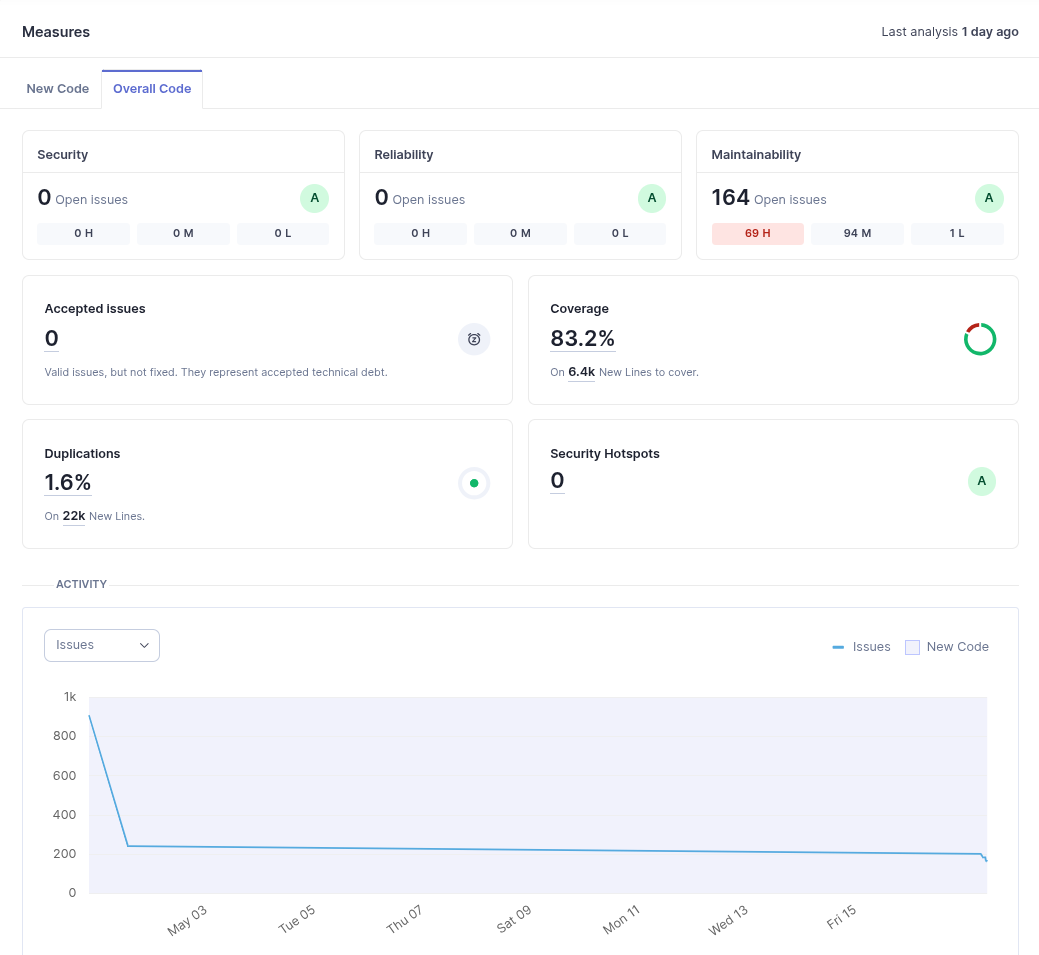
\includegraphics[width=0.95\textwidth]{captures/sonarqube_dashboard.png}
    \caption{Tableau de bord SonarQube -- métriques de qualité de RevMine}
    \label{fig:sonar-dashboard}
\end{figure}

% ------------------------------------------------------------
\subsection{Résultats et couverture}
% ------------------------------------------------------------

La Figure~\ref{fig:tests-passed} présente les résultats d'exécution de l'ensemble des tests
pytest, confirmant que tous les services passent l'intégralité de leur suite de tests.

\begin{figure}[H]
    \centering
    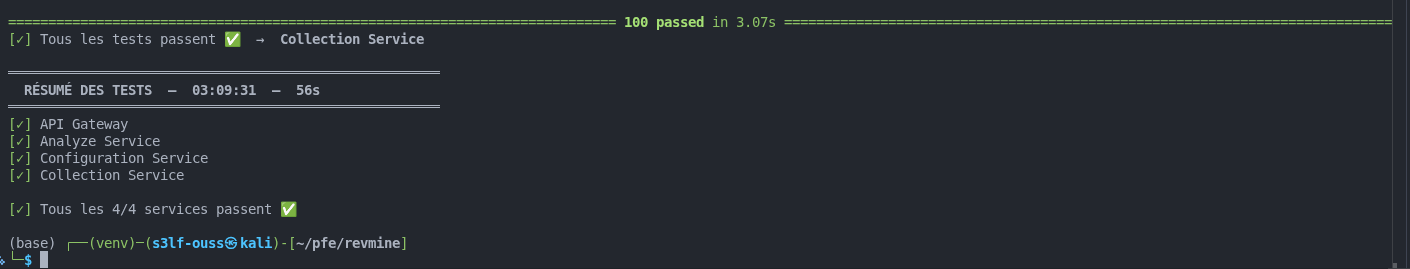
\includegraphics[width=0.95\textwidth]{captures/pytest_results_passed.png}
    \caption{Résultats d'exécution des tests pytest -- tous les services (tous les tests réussis)}
    \label{fig:tests-passed}
\end{figure}

Les données de couverture disponibles pour les services analysés via les rapports Cobertura sont
rassemblées dans le Tableau~\ref{tab:couverture}.

\begin{table}[H]
\centering
\small
\caption{Taux de couverture des tests unitaires par service}
\label{tab:couverture}
\begin{tabular}{|>{\raggedright\arraybackslash}p{4.5cm}
                |>{\centering\arraybackslash}p{3.2cm}
                |>{\centering\arraybackslash}p{3.2cm}
                |>{\centering\arraybackslash}p{2.8cm}|}
\hline
\textbf{Service} & \textbf{Lignes valides} & \textbf{Lignes couvertes} & \textbf{Couverture} \\
\hline
Service de passerelle d'API & 1\,568 & 909 & \textbf{57,97\,\%} \\
\hline
Service de configuration & \textit{en cours} & \textit{en cours} & \textit{en cours} \\
\hline
Service de collecte & \textit{en cours} & \textit{en cours} & \textit{en cours} \\
\hline
Service d'analyse & \textit{en cours} & \textit{en cours} & \textit{en cours} \\
\hline
\end{tabular}
\end{table}

Une synthèse globale des tests réalisés sur la plateforme, par service et par couche, est
proposée dans le Tableau~\ref{tab:recap-tests}.

\begin{table}[H]
\centering
\small
\caption{Récapitulatif des tests par service et par couche}
\label{tab:recap-tests}
\begin{tabular}{|>{\raggedright\arraybackslash}p{4cm}
                |>{\centering\arraybackslash}p{3cm}
                |>{\raggedright\arraybackslash}p{6cm}|}
\hline
\textbf{Service / Couche} & \textbf{Fichiers de tests} & \textbf{Portée principale} \\
\hline
Service de passerelle d'API & 1 & Robustesse du pipeline CI \\
\hline
Service de configuration & 7 & Domaine, infrastructure, API, Kafka \\
\hline
Service de collecte & 6 & API, domaine, services, intégration \\
\hline
Service d'analyse & 9 & Métriques, datasets, API, Celery \\
\hline
Frontend (Jest) & 1+ & Services HTTP, composants React \\
\hline
Frontend (Cypress) & 3 & Scénarios E2E complets \\
\hline
Service LLM & 500~scénarios & Parsing langage naturel, conformité au schéma JSON \\
\hline
\end{tabular}
\end{table}

% ============================================================
\section{Déploiement et pipeline CI/CD}
% ============================================================

\subsection{Pipeline GitLab CI}

Le pipeline d'intégration et de livraison continues (CI/CD\footnote{CI/CD~: \textit{Continuous
Integration / Continuous Delivery}. L'intégration continue consiste à automatiser la vérification
du code à chaque modification~; la livraison continue étend cette automatisation jusqu'à la
construction des livrables déployables.}) de RevMine est défini dans le fichier
\texttt{.gitlab-ci.yml}. Il s'organise en trois étapes successives~: \textbf{test},
\textbf{qualité} et \textbf{build}, dont les responsabilités sont détaillées dans le
Tableau~\ref{tab:pipeline-ci}.

\begin{table}[H]
\centering
\small
\caption{Étapes du pipeline GitLab CI de RevMine}
\label{tab:pipeline-ci}
\begin{tabular}{|>{\raggedright\arraybackslash}p{2cm}
                |>{\raggedright\arraybackslash}p{4.5cm}
                |>{\raggedright\arraybackslash}p{6.5cm}|}
\hline
\textbf{Étape} & \textbf{Job(s)} & \textbf{Description} \\
\hline
\texttt{test} & \texttt{test:all} & Exécution des tests unitaires de tous les services backend \\
\hline
\texttt{quality} & \texttt{sonar:scan} & Analyse SonarQube et validation du Quality Gate \\
\hline
\texttt{build} & \makecell[l]{\texttt{build:api-gateway} \\ \texttt{build:analyze} \\ \texttt{build:configuration} \\ \texttt{build:collection}} & Construction des images Docker (branches \texttt{main}/\texttt{master} uniquement) \\
\hline
\end{tabular}
\end{table}

\paragraph{Étape de test.} Le job \texttt{test:all} s'exécute sur une image
\texttt{python:3.11-slim} avec un service PostgreSQL~15 comme base de données de test. Il
provisionne les quatre bases de données nécessaires (\texttt{gateway\_db}, \texttt{analyze\_db},
\texttt{configuration\_db}, \texttt{collection\_db}), puis lance séquentiellement les tests pour
chaque service backend. Pour chaque service, les dépendances Python sont installées dans un
environnement virtuel dédié, et pytest génère les rapports JUnit (\texttt{junit-report.xml}) et
Cobertura (\texttt{coverage.xml}), conservés comme artefacts dans l'interface GitLab pendant
une semaine.

\paragraph{Étape d'analyse qualité.} L'étape \texttt{quality} exécute le scanner SonarQube en
s'appuyant sur les rapports de couverture générés lors de l'étape précédente. Le Quality Gate
bloquant interrompt le pipeline si les seuils ne sont pas atteints.

\paragraph{Étape de build Docker.} Déclenchée uniquement sur les branches \texttt{main} ou
\texttt{master}, elle construit les images Docker pour les quatre services backend principaux,
chacun disposant de son propre \texttt{Dockerfile} basé sur \texttt{python:3.11-slim}.

Les Figures~\ref{fig:pipeline-passed} et~\ref{fig:pipeline-failed} illustrent respectivement
une exécution réussie et un exemple d'échec détecté par le pipeline.

\begin{figure}[H]
    \centering
    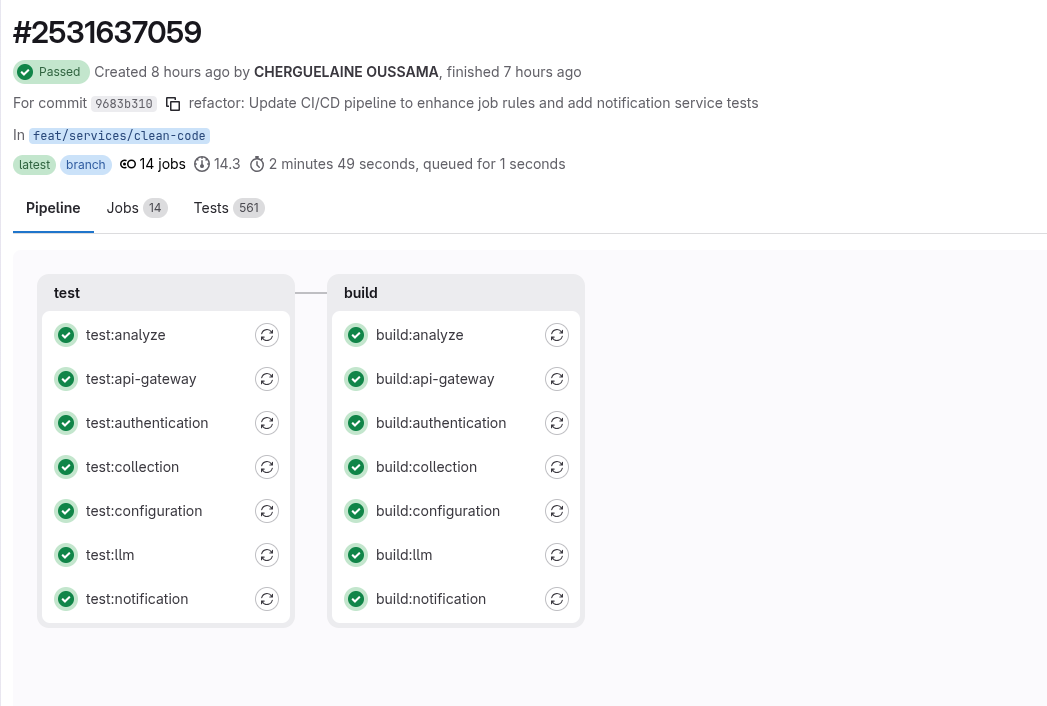
\includegraphics[width=0.95\textwidth]{captures/gitlab_pipeline_passed.png}
    \caption{Pipeline GitLab CI -- exécution réussie (toutes les étapes validées)}
    \label{fig:pipeline-passed}
\end{figure}

\begin{figure}[H]
    \centering
    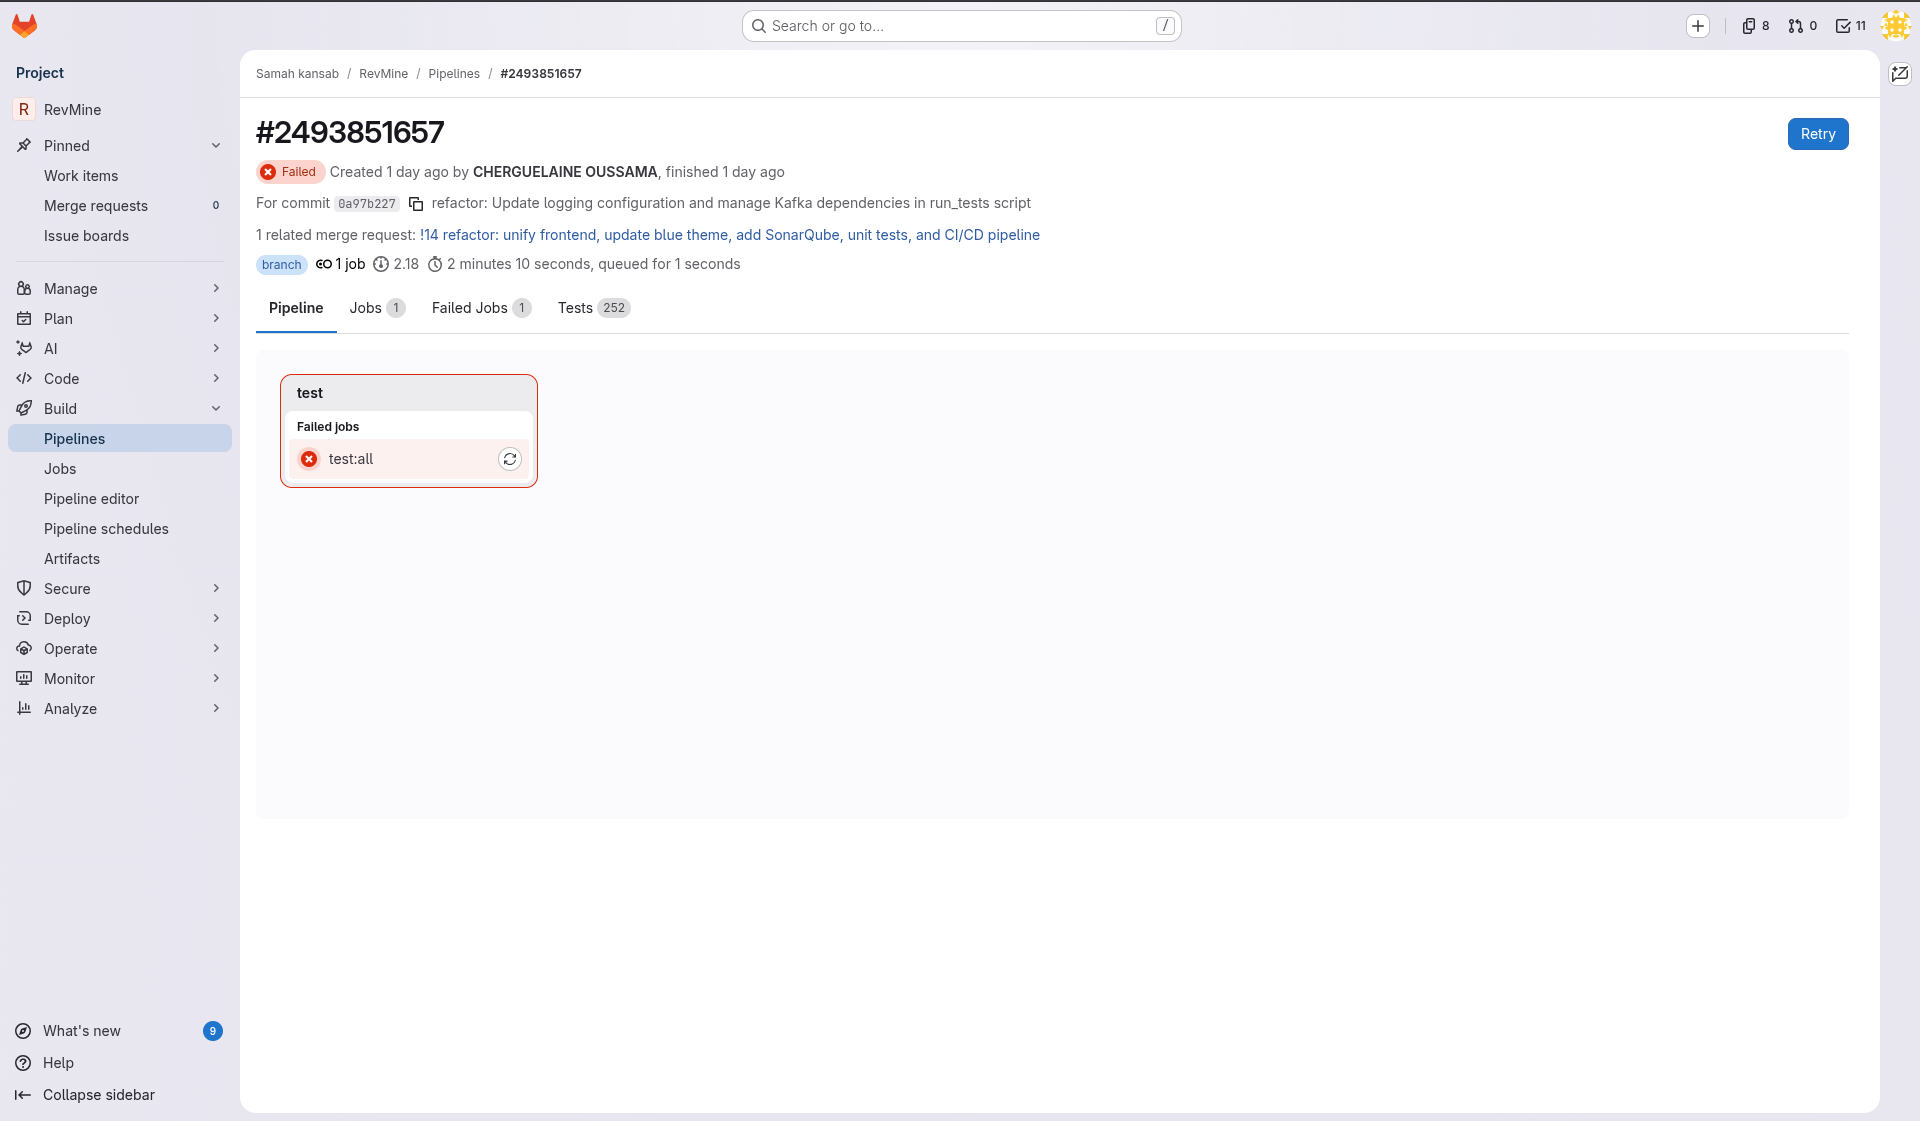
\includegraphics[width=0.95\textwidth]{captures/gitlab_pipeline_failed.png}
    \caption{Pipeline GitLab CI -- exemple d'échec détecté par le pipeline}
    \label{fig:pipeline-failed}
\end{figure}

\subsection{Déploiement avec Docker Compose}

En environnement de développement et de test, le déploiement de l'ensemble de la plateforme est
assuré par \textbf{Docker Compose}. Le fichier \texttt{docker-compose.yaml} orchestre le
démarrage synchronisé de tous les conteneurs~:

\begin{itemize}
    \item les quatre bases de données PostgreSQL~15~;
    \item Apache Kafka en mode KRaft (Confluent Platform 7.5.0)~;
    \item MinIO pour le stockage objet compatible S3~;
    \item la pile d'observabilité Loki + Promtail + Grafana~;
    \item les services applicatifs backend et le frontend React.
\end{itemize}

Un réseau Docker commun assure la communication entre les conteneurs. Des volumes persistants
sont définis pour les bases de données et MinIO, garantissant la conservation des données entre
les redémarrages.

% ============================================================
\section{Limites et perspectives}
\label{sec:limites}
% ============================================================

Bien que la démarche de réalisation et de test mise en place soit solide, plusieurs limites ont
été identifiées~:

\begin{itemize}
    \item \textbf{Couverture partielle du service de passerelle d'API}~: avec 57,97\,\% de
          couverture, certaines branches de code -- notamment celles liées aux fournisseurs OAuth
          et aux orchestrateurs -- ne sont pas entièrement testées~;
    \item \textbf{Tests d'intégration inter-services}~: les interactions entre microservices via
          Kafka n'ont pas toutes été validées dans un environnement d'intégration complet~; un
          environnement de test Kafka dédié (par exemple via \textit{testcontainers}) serait
          nécessaire pour couvrir l'ensemble des scénarios de messagerie~;
    \item \textbf{Absence de tests de charge}~: aucun test de performance n'a été réalisé pour
          évaluer le comportement de la plateforme sous forte sollicitation~;
    \item \textbf{Service de notification sans couverture formelle}~: le service Go ne dispose
          pas encore d'une suite de tests automatisée~; son fonctionnement est validé
          indirectement via les scénarios Cypress et l'observation des événements WebSocket~;
    \item \textbf{Évaluation LLM hors pipeline CI}~: le benchmark statique n'est pas encore
          intégré au pipeline CI/CD, en raison des coûts d'inférence et de la nature non
          déterministe des sorties.
\end{itemize}

Afin de renforcer la couverture et la fiabilité, plusieurs améliorations sont envisageables~:
mise en place de tests d'intégration Kafka via \textit{testcontainers}, augmentation de la
couverture du service de passerelle d'API au-delà de 80\,\%, ajout de tests de charge via
\textit{Locust} ou \textit{k6}, création de suites de tests dédiées pour le service LLM et le
service de notification, et intégration de tests de sécurité automatisés (DAST/SAST) dans le
pipeline CI/CD.

% ============================================================
\section{Conclusion}
% ============================================================

La phase de réalisation de RevMine a permis de concrétiser l'architecture microservices définie
lors de la conception en une solution fonctionnelle, modulaire et évolutive. Développé en binôme,
le projet a bénéficié d'une organisation rigoureuse~: convention de branches justifiée, revues de
code systématiques, sprints hebdomadaires et réunions mensuelles avec l'encadrant de l'ETS.

Le choix de technologies complémentaires et adaptées à chaque périmètre -- Python/Django pour les
services métier, FastAPI pour le service LLM, Go pour les notifications temps réel, React pour
le frontend, et la pile Grafana/Loki/Promtail pour l'observabilité -- a permis de répondre aux
exigences de performance, de maintenabilité et de flexibilité.

La culture DevOps adoptée, matérialisée par le pipeline GitLab CI avec Quality Gate SonarQube
bloquant, garantit qu'aucun code dégradé ne passe en intégration. La communication asynchrone
via Kafka et la conteneurisation complète via Docker assurent une plateforme robuste et
reproductible dans différents environnements.

Enfin, la stratégie de test multi-niveaux -- des tests unitaires aux scénarios end-to-end en
passant par l'évaluation empirique du service LLM sur 500~scénarios -- pose les fondements d'une
plateforme fiable et maintenable, capable d'intégrer de nouvelles fonctionnalités sans compromettre
la qualité de l'existant.